\documentclass[11pt]{article}
\usepackage[margin=1in]{geometry}
\usepackage{amsmath,amssymb,mathtools}
\usepackage{booktabs}
\usepackage{xcolor}
\usepackage{tikz}
\usepackage[colorlinks=true,linkcolor=blue!50!black,citecolor=blue!50!black,urlcolor=blue!50!black]{hyperref}

\colorlet{wire}{blue!60!cyan!80!black}
\colorlet{dial}{orange!85!black}

\title{Local work is free, connections cost:\\ the exponent $9/4$ and the CX lower bound}
\date{Working notes, November 24, 2026}

\begin{document}
\maketitle

\section*{The analogy}

Picture a few teams working in separate rooms. Anything a team does inside its own room is free.
The only thing that costs money is a phone line between two rooms. The question is how small the
phone bill can be for a given job.

Both results are about this phone bill.
\begin{itemize}
\item \textbf{Matrix multiplication}~\cite{mm94}. The rooms are the three tensor factors $A,B,C$.
  Free work means local linear maps. The bill is the rank $r$, and a rank-$r$ algorithm amounts to
  one shared line with $r$ values (Fig.~\ref{fig:rooms}, left).
\item \textbf{CX synthesis}~\cite{smb2q}. The rooms are the qubits. Free work means single-qubit
  gates. The bill is the CX count, and each CX is a one-bit line between two qubits: the control
  copies its bit and the target XORs it in (Fig.~\ref{fig:rooms}, right).
\end{itemize}
A lower bound in either setting has the same shape:
\[
\#\text{lines}\ \ge\ \frac{\text{what the job demands}}{\text{what one line supplies}} .
\]
The two results differ in \emph{what} the job demands, and that difference explains why each
answer looks the way it does.

\begin{figure}[h]
\centering
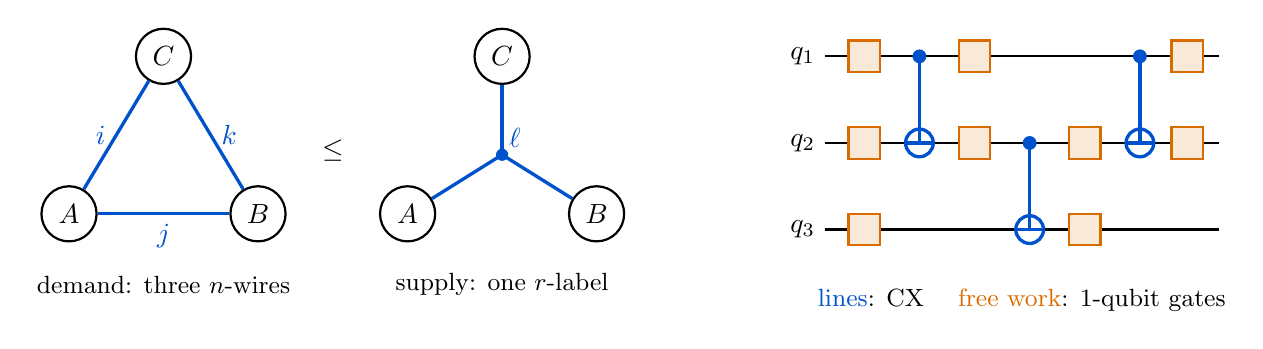
\begin{tikzpicture}[site/.style={circle,draw,thick,minimum size=7mm,inner sep=0pt}]
  % --- matrix multiplication: three indices vs one shared label
  \begin{scope}
    \node[site] (A) at (0,0) {$A$};
    \node[site] (B) at (2.4,0) {$B$};
    \node[site] (C) at (1.2,2.0) {$C$};
    \draw[wire,very thick] (A) -- node[below] {$j$} (B);
    \draw[wire,very thick] (B) -- node[right] {$k$} (C);
    \draw[wire,very thick] (C) -- node[left] {$i$} (A);
    \node at (1.2,-0.9) {\small demand: three $n$-wires};
  \end{scope}
  \node at (3.35,0.8) {$\le$};
  \begin{scope}[xshift=4.3cm]
    \node[site] (A2) at (0,0) {$A$};
    \node[site] (B2) at (2.4,0) {$B$};
    \node[site] (C2) at (1.2,2.0) {$C$};
    \coordinate (L) at (1.2,0.75);
    \fill[wire] (L) circle (2.2pt) node[above right=-1pt] {$\ell$};
    \draw[wire,very thick] (L) -- (A2);
    \draw[wire,very thick] (L) -- (B2);
    \draw[wire,very thick] (L) -- (C2);
    \node at (1.2,-0.9) {\small supply: one $r$-label};
  \end{scope}
  % --- CX circuit: qubits as rooms, CX as one-bit lines, 1q gates as dials
  \begin{scope}[xshift=9.6cm,yshift=-0.2cm]
    \foreach \y/\q in {2.2/1,1.1/2,0/3} {
      \draw[thick] (0,\y) -- (5,\y);
      \node[left] at (0,\y) {$q_\q$};
    }
    \foreach \x/\y in {0.5/2.2,0.5/1.1,0.5/0, 1.9/2.2,1.9/1.1, 3.3/1.1,3.3/0, 4.6/2.2,4.6/1.1} {
      \node[draw=dial,fill=dial!15,thick,minimum size=4mm,inner sep=0pt] at (\x,\y) {};
    }
    % CX gates
    \foreach \x/\yc/\yt in {1.2/2.2/1.1, 2.6/1.1/0, 4.0/2.2/1.1} {
      \draw[wire,very thick] (\x,\yc) -- (\x,\yt);
      \fill[wire] (\x,\yc) circle (2.5pt);
      \draw[wire,very thick] (\x,\yt) circle (5pt);
      \draw[wire,very thick] (\x-0.18,\yt) -- (\x+0.18,\yt);
    }
    \node at (2.5,-0.9) {\small \textcolor{wire}{lines}: CX \quad \textcolor{dial}{free work}: 1-qubit gates};
  \end{scope}
\end{tikzpicture}
\caption{Left: $T_n$ needs three index wires $i,j,k$ between the rooms, and a rank-$r$ algorithm
must supply them from one shared label (after Fig.~1 of~\cite{mm94}). Right: a CX circuit, with
qubits as rooms, CX gates as one-bit lines and single-qubit gates as free local work.}
\label{fig:rooms}
\end{figure}

\section*{Two kinds of demand}

There are two reasons a job might need many phone calls.

\paragraph{The teams must share a lot of information.} In $T_n$, rooms $A$ and $B$ have to agree
on an index $j$ with $n$ values, $B$ and $C$ on $k$, and $C$ and $A$ on $i$. The preprint puts a
price on such agreement: a geometry in which each line has a length. In the geometry it chooses,
the three wires cost a total of $6\log n$, while one shared label of size $r$ supplies only
$\tfrac83\log r$. That gives
\[
6\log n\ \le\ \tfrac83\log r \quad\Longrightarrow\quad r\ \ge\ n^{9/4}.
\]

\paragraph{The teams must receive many independent instructions.} A generic unitary is specified
by $4^n$ real numbers. All of those numbers have to live in the dials of the single-qubit gates.
However, two dials in the same room with no call between them merge into a single dial. Each CX
therefore opens room for only four new real parameters. That gives
\[
4\,c+3n+1\ \ge\ 4^n \quad\Longrightarrow\quad c\ \ge\ \tfrac14\big(4^n-3n-1\big).
\]

\section*{Why each problem is driven by a different demand}

\begin{center}
\begin{tabular}{@{}lll@{}}
\toprule
 & matrix multiplication & CX synthesis \\
\midrule
target & one fixed tensor $T_n$ & a generic $U$ \\
instructions to deliver & none: $T_n$ has no free parameters & $4^n$ \\
information to share & large: three $n$-valued indices & at most $O(n^2)$ CX worth \\
bound comes from & information & instructions \\
open question & settled: $\omega=9/4$ & the constant in $[\tfrac{12}{48},\tfrac{21}{48}]$ \\
\bottomrule
\end{tabular}
\end{center}

$T_n$ is a single fixed tensor with no dials to set. Counting instructions therefore gives nothing,
and the whole difficulty lies in pricing information. The $9/4$ theorem answers exactly that.

Generic $U$ is the opposite case: it is all dials. The information it forces across the rooms is
small. Under any price of the preprint's kind, each CX carries one bit along one line, and the
total demand is capped by the rank of $U$ (at most $4^{n-1}$) and by how cheaply a tree of lines
can build a shared label. Together these give at most $2(n-1)^2$ CX gates, which is why the
operator-Schmidt-rank bound stops at $n$. The $4^n$ comes entirely from the instructions.

The upshot is that the two problems share one ledger and use different currencies. The preprint is
a powerful new way to price \emph{shared information}, and it says nothing new about delivering
\emph{instructions}. Closing the gap between the pivot count $\tfrac{21}{48}4^n$ and
$\tfrac14 4^n$ means doing the instruction count more carefully. One could ask which dials are
redundant at a generic circuit, or how many circuits reach the same $U$. A sharper price of the
preprint's kind would not help.

\begin{thebibliography}{9}
\bibitem{mm94} OpenAI, \emph{The matrix multiplication exponent is nine fourths}, preprint,
  November 24, 2026,
  \url{https://github.com/openai/math/blob/main/preprints/The-matrix-multiplication-exponent-is-nine-fourths-November-24-2026/paper.pdf}.
\bibitem{smb2q} V.~V.~Shende, I.~L.~Markov, S.~S.~Bullock, \emph{Minimal universal two-qubit
  controlled-NOT-based circuits}, Phys.\ Rev.\ A \textbf{69}, 062321 (2004).
\end{thebibliography}

\end{document}
